\chapter{Recommender methods}
\label{recommender_methods}
\thispagestyle{empty}

In this chapter we discuss at length the various recommender systems we choose to drive the recommendation of nodes in our networks. These recommender systems form the crux of our experiments, as in we use them to analyze the bias existing in the recommendations provided by them. In the following chapters we abstract out these systems by the notation $R$.

We can divide the methods we use in two groups. In the first group we exclusively talk about systems which provide recommendations based on the network topology and/or node attributes. We call these set of methods \textbf{Topological methods}. In the second group we take into consideration the set of methods which are based on reinforcement learning. These are methods which learn the behaviour of node selection from the system users and use this learning to provide recommendations later, thus reinforcing its perception. We call these set of methods \textbf{Reinforcement methods}.

In chapters \ref{analysis_chapter} and \ref{case_study} we see how these methods are used in the context of our thesis to solve the research goals we had defined previously in \ref{research_goals}. 

While outlining the methods below, we define the setting as having a network $G_{i}(V_{i}, E_{i})$ at timestamp $i$, where $V_{i}$ is the node set and $E_{i}$ is the undirected edge set for network $G_{i}$. We consider a specific node $v \in V_{i}$ for which we wish to receive a recommendation list $L_{v}$ of length $k$. We also define $V^{\prime}_{i}(v)=\{u | u \in V_{i} \land u \ne v \land (u,v) \notin E_{i}\}$ as the set of vertices which are not already connected with $v$ in the network instance $G_{i}$. Now that we have formally defined our setting, we start describing the workings of each method in detail. 

\section{Topological Methods}
In this section we discuss about the set of different recommendation algorithms which carry out their vocation based on the network topology and/or node attributes. We talk about three such methods which we have taken into consideration in our thesis and lay down the steps followed by each of these methods. 

\subsection{Preferential Attachment with Homophily}
We use the probability value in preferential attachment with homophily model \cite{karimi2018homophily} as a measure to rank nodes among themselves, using this as a recommendation mechanism. 

We construct the recommendation list $L_{v}=(u_{1},...,u_{k} | u_{*} \in V^{\prime}_{i}(v))$ for the node $v$ by computing the probability values for all nodes $u \in V^{\prime}_{i}(v)$ according to equation \ref{preferential_homo_eqtn}, where $\delta(x)$ denotes the current degree of the node $x$ and $h_{xy}$ denotes the homophily value between nodes $x$ and $y$.

\begin{equation}
\label{preferential_homo_eqtn}
\Pi_{u} = (\delta(u) \times h_{uv}) / \sum_{w \in V^{\prime}_{i}(v)}^{} (\delta(w) \times h_{wv})
\end{equation}

The nodes are ranked according to their probability measure $\Pi_{u}$ from highest to lowest, and the final list $L_{v}$ is formed by taking the first $k$ items from this ranked formation.

\subsection{Adamic-Adar Index}
The Adamic-Adar Index \cite{adamic2003friends} was proposed by Adamic et. al. in 2003. To establish it as a good contender among recommendation algorithms we cite the study conducted by Liben-Nowell et. al., where this, along with other link prediction methods were used on empirical co-authorship networks, and it was found that: Adamic-Adar Index, despite being simple, performed best amongst others \cite{liben2007link}.

Through this index, similarity between two nodes in a network is derived by considering the amount of shared commonalities among them (in our case, shared connections; although, this might mean other attributes for different kinds of networks). The idea originates from the notion of triadic closure of nodes in a network. The index considers a common node to have higher importance in the final calculation of the index if this node has fewer connections, signifying that this node has slightly exclusive connections or exhibits esoteric properties.

For all $u \in V^{\prime}_{i}(v)$ we compute the Adamic-Adar Index according to the equation \ref{adamic_eqtn}, where $\Gamma(x)=\{w | w \in V_{i} \land (w,x) \in E_{i}\}$ denotes the neighbors for $x$. 

\begin{equation}
\label{adamic_eqtn}
AAI(u,v) = \sum_{w \in \Gamma(u) \cap \Gamma(v)}^{} \frac{1}{log(|\Gamma(w)|)}
\end{equation}

The nodes are ranked in descending order of the index value $AAI$ and the first $k$ nodes form the recommendation list $L_{v}$.

\subsection{Twitter Ranking}
The ranking architecture of Who-To-Follow feature in Twitter is powered by this method \cite{gupta2013wtf}. A bipartite graph is composed from the network. This bipartite graph is composed of hubs and authorities. A SALSA \cite{lempel2001salsa} scoring mechanism is used on these hubs and authorities to rank the nodes. We follow the steps similar to that which has been outlined by Gupta et. al. in \cite{gupta2013wtf}, with slight modifications to scale down to our requirements. We detail the steps followed in twitter ranking below.

\begin{enumerate}
	\item A ``circle of trust'' is formed for the node $v$ by computing personalized PageRank scores for the nodes in $V^{\prime}_{i}(v)$. We limit the number of nodes in this circle of trust to $k$. In the original paper the number of nodes considered in the ``circle of trust'' is 500, however we scale down to be the number of recommendations we are seeking considering the small size of our network and also for only the top-most results. Nodes in the ``circle of trust'' is termed as \textbf{hub} nodes, denoted by $H_{v}$.
	
	\item We construct the \textbf{authorities} nodes set $A_{v}$ by considering the nodes from $V^{\prime}_{i}(v)$ which have an edge with the nodes present in $H_{v}$.
	
	\item We construct a bipartite graph with $H_{v}$ on one side and $A_{v}$ on the other side. We put edges between the hubs and the authorities as found in $E_{i}$. Since it is a bipartite graph, there are no edges among nodes in $H_{v}$ or among nodes in $A_{v}$.
	
	\item Upon construction of the bipartite graph, we use SALSA \cite{lempel2001salsa} to rank all the nodes in $\{H_{v} \cap A_{v}\}$ according to their SALSA scores.
	
	\item From this ranked order of nodes, the first $k$ nodes form $L_{v}$. 
	
\end{enumerate}

\section{Reinforcement Methods}

In this section we outline the set of recommendation algorithms which use reinforcement learning techniques, specifically Learning-To-Rank mechanisms to rank nodes for recommendations. 

In reinforcement learning algorithms, an agent learns which actions to take based on the feedback it receives from its environment. The recommender system is our agent here which learns from the feedback it receives from the activities of the \textbf{Click Model}. We start by defining the click model, which we would be using to drive the training of our learning model. Once we have established it, we highlight the two Learning-To-Rank methods which we use in our thesis. 

As we have also mentioned in Chapter \ref{chapter_background}, Learning-To-Rank methods were developed primarily for the ranking of search query results. Since network recommenders do not use reinforcement methods as far as we know, we adapted these algorithms from the search-query domain into ours. When we write down the details for these algorithms we will thus be writing them in the context of networks and recommendations, which is different from that what is presented in the original papers, which interested readers can find from given citations.

\subsection{Click Model}
\label{click_model}

We need a model which can give us perspective of how nodes choose to form links in real scenarios. In real-world, networks may be formed owing to various factors. We need a suitable abstraction as our model which can act as an agent aiding training for our reinforcement methods.

Due to lack of data on how nodes choose to form edges in real-world we cannot train using a specific dataset, which is the preferred methodology. Given that the preferential attachment with homophily model \cite{karimi2018homophily} has been proved successful in explaining empirical networks we consider this model largely as our click model to mirror edge-formation behaviour. 

We refer to our click model as $C$ in the subsequent text. At each training iteration, the click model is presented with the node $v$ as the perspective node for which the click decisions would be taken and a list of nodes $L_{v}=(u_{1},...u_{k} | u_{*} \in V^{\prime}_{i})$. The click model calculates probability $\alpha_{v}(u_{j}), \forall u_{j} \in L_{v}$. These probability values are used for choosing a candidate clicked node from the set of nodes in $L_{v}$ using equation \ref{click_model_eqtn}. In the given equation, $\delta(x)$ denotes the degree of node x and $h_{xy}$ denotes the homophily value among the nodes $x$ and $y$.

\begin{equation}
\label{click_model_eqtn}
\alpha_{v}(u_{j+1}) = \frac{\delta(u_{j+1}) \times h_{u_{j+1}v} \times e^{(1-j)\times r^{2}}}{\sum_{m=0}^{k-1} \delta(u_{m+1}) \times h_{u_{m+1}v} \times e^{(1-m)\times r^{2}}}
\end{equation} 

In equation \ref{click_model_eqtn} we also come across the parameter $r$, which we define as the ranking factor, whose value can range between $[0,1]$. This tuneable parameter signifies how much effect the rank $j$ of a node $u_{j} \in L_{v}$ has effect in the calculation of probability $\alpha_{v}(u_{j})$. For a value of $r=0$, all nodes in the list $L_{v}$ are considered of equal importance and hence the placement in the list does not have any effect. For a value of $r=1$, the ranking of a node has a very strong effect in boosting the node's selection probability. We can see the effect of $r$ in different ranking indexes in figure \ref{ranking_factor_fig}.

\begin{figure}[h]
	\centering
	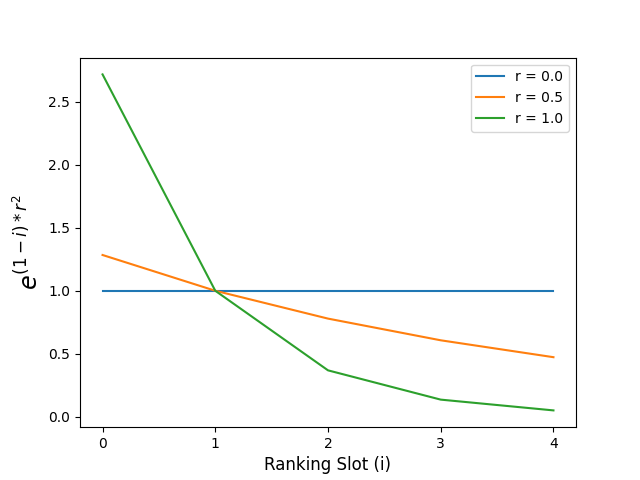
\includegraphics[width=0.7\textwidth]{images/ranking_factor.png}
	\caption{Effect of Ranking Factor}
	\label{ranking_factor_fig}
\end{figure}

\subsection{Ranked Bandits}

The Ranked Bandits algorithm \cite{radlinski2008learning} was developed by Radlinski et. al. in 2008. This was one of the first successful model for ranking search query results using reinforcement learning techniques. 

\textbf{Multi-Armed Bandits} is a classic reinforcement learning problem which deals with how to maximize the reward outcome in a given scenario based on the given choice of actions and the benefit/drawback associated with each making a choice only known partially to the algorithm. This is a typical explore-exploit scenario, where the agent wants to explore new choices in the action space for different scenarios, but also wants to have a conservative approach to maximize its rewards based on actions it takes. This balancing act is carried out in several different ways by different Multi-Armed Bandit algorithms.

Below we outline the steps taken by Ranked Bandits to train and ultimately provide a list $L_{v}$ for a given node $v$. 

\begin{enumerate}
	\item $k$ Multi-Armed Bandits $(MAB_{1},...,MAB_{k})$ are initialized for $k$ ranking slots. Each $MAB_{j}$ is responsible for suggestion of the node at the $j$-th index in $L_{v}$. The $MAB$s internally uses the Exp3 algorithm \cite{auer2002nonstochastic} for making an action choice (in this case choosing a node from the list of nodes in $V^{\prime}_{i}$). Exp3 was found to perform better by Radlinski et. al., and hence we choose the same for our purpose.
	
	\item At each training iteration, each $MAB_{j}$ is queried for the best node suggestion at index $j$ with reference to the seeking node $v$. The $MAB$s are queried in order, from $0$ to $k$. If $MAB_{j}$ suggests node $u_{j}$, then a check is made to see if this node was previously suggested by any other $MAB_{<j}$ for that training iteration. In case, that happens then a random node is chosen among the list of available nodes in $V^{\prime}_{i}$ and put as $u_{j}$.
	
	\item The recommendation list $L_{v}=(u_{1},..u_{k})$ is provided to the click model $C$, and a bitset $B=(b_{0},...,b_{k})$ is returned by $C$ where $b_{*}$ is either marked as 0 or 1, signifying whether the node was chosen by $C$ or not.
	
	\item If $u_{j}$ in $L_{v}$ was originally suggested by $MAB_{j}$ and $C$ chose it, then a reward of 1 is provided to the $MAB_{j}$ for suggesting that node. Else a reward of 0 is given to the $MAB_{j}$. With the reward values, the $MAB$s adjust their internal action specific gains which leads to better future predictions.
\end{enumerate}

\subsection{Top Rank}

Top Rank \cite{lattimore2018toprank} was developed by Lattimore et. al. in 2018. Earlier algorithms used to have mostly offline training mechanisms, whereas this was the first algorithm to make the learning process continuous (online learning). The basic idea of the algorithm is to maintain partial sets of nodes with preference ranking amongst these sets according to the feedback it receives by observing clicks. It keeps updating these partial set elements upon receiving feedback about them such that items in a higher set are always known to have better reward on selection. 

A broad overview of the steps taken by Top Rank is given below. 

\begin{enumerate}
	\item A partition set $P=\{P_{0}\}$ is initially created, where $P_{0}$ contains all nodes in $V^{\prime}_{i}$. 
	
	\item $k$ nodes are selected at each training iteration from the partitions in $P$. Partitions are ranked according to their index, so $P_{0}$ has a higher preference over $P_{1}$, which has higher preference over $P_{2}$, and so on. All nodes belonging to a certain partition have the same preference. A list $L_{v}=(u_{1},..u_{k} | u_{*} \in V^{\prime}_{i}(v))$ is created from the partitions in $P$, chosen according to precedence. Nodes from the same partition are always selected randomly, and the next partition is considered for node selection only when the previous one has been exhausted and the $L_{v}$ list still has less than $k$ nodes. 
	
	\item The $L_{v}$ list, upon creation, is provided to the click model $C$ which returns a bitset $B=(b_{0},...,b_{k})$ where $b_{*}$ is either 0 or 1, signifying whether the node at that position was chosen by $C$ or not.
	
	\item Using the feedback received from $C$ it is determined whether the existing partitions in $P$ can be broken down further based on the confidence of a node being placed in a higher preference partition or being demoted down to a lower partition. The details of the calculation which aids this decision can be found in the original paper \cite{lattimore2018toprank}.
	
	\item Steps 2-4 are repeated for all the training iterations. Finally we get the complete node set $V^{\prime}_{i}$ divided into partitions $P$ ranked according to preference.
	
	\item The Partition sets $P$ is used to get node recommendations in the same way as step 2 suggests.
	
\end{enumerate}

\section{Summary}

We end the chapter with a brief summary of all the recommendation methods which we would be using in the subsequent chapters and will be abstracting as $R$. We also introduce the short keyword names for the methods as \textbf{bolded text} here, which we use in the future chapters: in plots and discussions.

\textbf{PA-Homophily}: The preferential attachment with homophily method uses the probability measure in Karimi's generative model \cite{karimi2018homophily} for node rankings and recommendations.

\textbf{Adamic-Adar}: The Adamic-Adar Index uses an index measure as defined by Adamic et. al. \cite{adamic2003friends}. It recommends nodes based on similarity of nodes in terms of neighbours they share.

\textbf{Twitter-Rank}: Ranking used by Twitter to drive Who-To-Follow \cite{gupta2013wtf}. Combines SALSA scoring and egocentric random walk methods to get a recommendation list.

\textbf{Ranked-Bandit}: Reinforcement Learning method which maintains different MABs for each index in the recommendation list \cite{radlinski2008learning}. Each MAB is responsible to recommend the best node for that index. The MABs use Exp3 internally to perform the explore-exploit balance of choosing nodes among the given choice-set.

\textbf{Top-Rank}: Reinforcement Learning method which maintains several partitions, which are ordered according to preference and contains a partial ranking of all nodes \cite{lattimore2018toprank}. The partitions are updated or nodes are moved among them on the basis of observation of clicking behavior. 